\documentclass[a4paper,11pt,bibliography=totoc, listof=totoc,titlepage]{scrartcl}
\usepackage[ngerman]{babel}
\usepackage[utf8]{inputenc}
\usepackage[left=3cm,right=2.5cm,top=2.5cm,bottom=2.5cm]{geometry}
\usepackage[onehalfspacing]{setspace}
\renewcommand{\arraystretch}{1.5}
\usepackage{graphicx}
\usepackage{color}
\usepackage[usenames,dvipsnames,table,xcdraw]{xcolor}
\usepackage[toc,page]{appendix}
%\usepackage[scaled]{berasans}
%\renewcommand*\familydefault{\sfdefault}  %% Only if the base font of the document is to be sans serif
%\usepackage[T1]{fontenc}

  
\usepackage[hyphens]{url}
\usepackage[hidelinks]{hyperref}
\usepackage{todonotes}
\usepackage{amsmath}

\usepackage{multirow}

\newcommand*\justify{%
  \fontdimen2\font=0.4em% interword space
  \fontdimen3\font=0.2em% interword stretch
  \fontdimen4\font=0.1em% interword shrink
  \fontdimen7\font=0.1em% extra space
  \hyphenchar\font=`\-% allowing hyphenation
}

\newcommand{\code}[1]{\texttt{\justify{#1}}}
%\usepackage{tocloft}

%Boxfehler
\hbadness=1000000

% Listings
\usepackage{listings}
\lstset{
   breaklines=true,
   captionpos=t,
   basicstyle=\scriptsize\ttfamily,
   keywordstyle=\bfseries\ttfamily\color{orange},
   stringstyle=\color{green}\ttfamily,
   commentstyle=\color{gray}\ttfamily,
   emph={square}, 
   emphstyle=\color{blue}\texttt,
   emph={[2]root,base},
   emphstyle={[2]\color{yac}\texttt},
   showstringspaces=false,
   flexiblecolumns=false,
   tabsize=2,
   numbers=left,
   numberstyle=\tiny,
   numberblanklines=false,
   stepnumber=1,
   numbersep=10pt,
   xleftmargin=15pt
 }

% Zitierstil
%\usepackage[style=authoryear,citestyle=authoryear,natbib=true]{biblatex}
%\bibliography{Thesis.bib}
\usepackage[round]{natbib}
\bibliographystyle{hcu}

\begin{document}
\pagenumbering{Roman}
\begin{titlepage}
\begin{center}
\renewcommand{\arraystretch}{0.7}
\begin{tabular}{lr}
\begin{tabular}{l}
\end{tabular} \hspace{0.5cm} &
\begin{tabular}{r}
Landesbetrieb Geoinformation und Vermessung\\
Neuenfelder Straße 19\\
21109 Hamburg\\
\end{tabular}
\end{tabular}\\\vspace{5cm}
\doublespacing 
{\huge\bfseries  QuerschnittsEditor
}\vspace{0.5cm}\\

{\large\bfseries Bedienerhandbuch
}\vspace{2cm}\\
{\large Florian Timm}\\

\vspace{10cm}
Stand: 14. Feb. 2020\\
\end{center}
\setcounter{page}{0} 
\end{titlepage}


% Mehrere gleichzeitig zitieren
\providecommand{\citeTwo}[4]{\citep[{\citealp[#1]{#2};}][#3]{#4}} 
\providecommand{\citeThree}[6]{\citep[{\citealp[#1]{#2}; \citealp[#3]{#4};}][#5]{#6}} 
\providecommand{\citeFour}[8]{\citep[{\citealp[#1]{#2}; \citealp[#3]{#4}; \citealp[#5]{#6};}][#7]{#8}}

\newpage

\tableofcontents
\newpage

\pagenumbering{arabic}
\setcounter{page}{1} 

\section{Grundlagen}
Der LGV-QuerschnittsEditor dient zur Bearbeitung von Querschnitten, Schildern und punktueller Straßenausstattung in der TTSIB. Er ermöglicht eine graphische Stationierung von Elementen, ohne das hierbei manuell Stationierungen festgelegt werden müssen.

\subsection{Login}
\begin{figure}
 \centering
 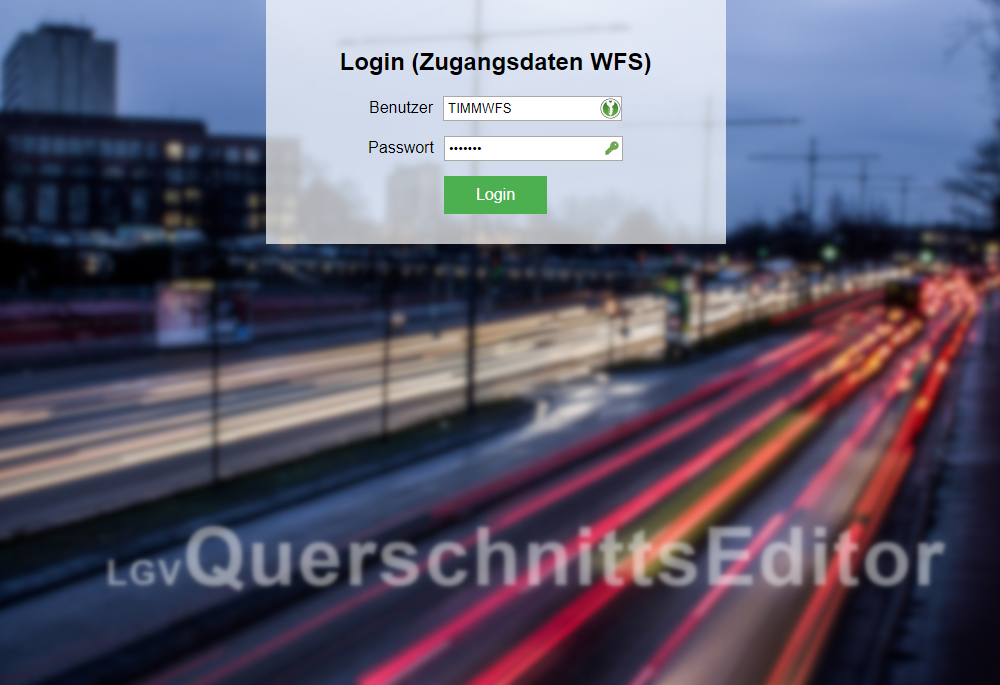
\includegraphics[width=.8\textwidth]{./img/login.png}
 \caption{Login-Oberfläche}
 \label{img:login}
\end{figure}

\label{ss:login}
Der Login (\autoref{img:login}) erfolgt mit Zugangsdaten des PublicWFS. Diese Zugangsdaten können, müssen aber nicht identisch sein mit den Zugangsdaten zu der TTSIB/INFOSYS und sind einzeln im Administratortool des PublicWFS anzulegen. 



\subsection{Auswahl des Ereignisraumes}

\begin{figure}
 \centering
 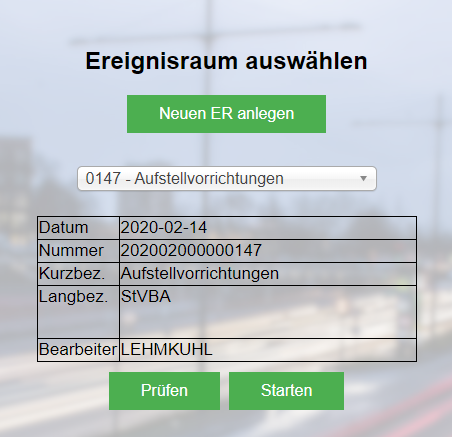
\includegraphics[width=.7\textwidth]{./img/er_auswahl.png}
 \caption{Auswahl des Ereignisraumes}
 \label{img:er_auswahl}
\end{figure}

Nach dem Login (siehe \autoref{ss:login}) öffnet sich die Auswahl des Ereignisraumes (\autoref{img:er_auswahl}). Hier ist es möglich bestehende Datenereignisräume auszuwählen, zu prüfen oder neue anzulegen. Durch Auswahl eines Ereignisraumes (ER) in der Drop-Down-Liste werden in der Tabelle hierunter die Informationen zu dem ausgewählten ER angezeigt. Durch einen Klick auf Starten wird der Ereignisraum über den PublicWFS geladen und die Objekte, die sich in dem Ereignisraum befinden geladen.



\subsection{Bearbeitungsmodus}
\begin{figure}
 \centering
 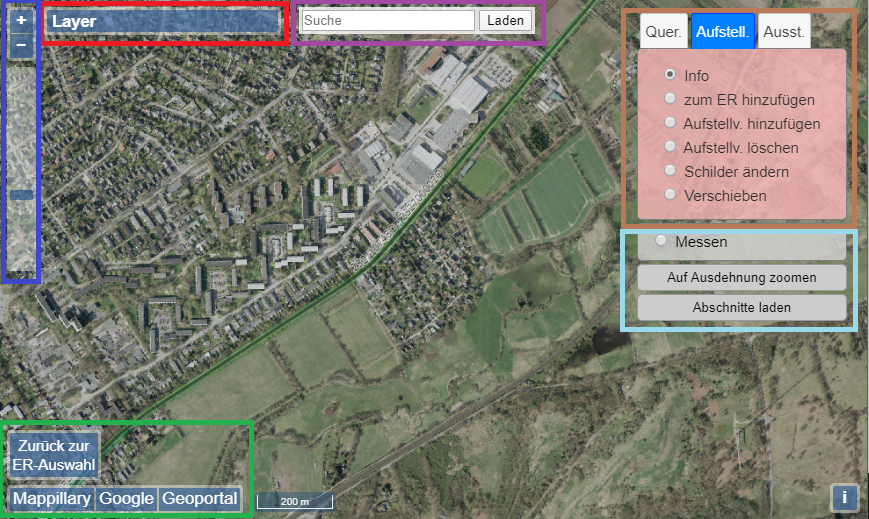
\includegraphics[width=.9\textwidth]{./img/bearbeitung.png}
 \caption{Bearbeitungsmodus}
 \label{img:bearbeitung}
\end{figure}
Wenn der Ereignisraum fertig geladen wurde, ist die Bearbeitung von Objekten möglich (\autoref{img:bearbeitung}). Wenn der Ereignisraum bereits Daten enthält, werden Straßenabschnitte und die Objekte angezeigt und auf diese gezoomt. Wenn keine Daten im Ereignisraum vorhanden sind, wird eine leere Karte angezeigt und eine Meldung angezeigt, dass keine Daten vorhanden sind.



\subsubsection{Kartensteuerung}
Die Karte wird mit der Maus gesteuert. Durch Klicken und Halten der linken Maustaste wird die Karte verschoben.Hineingezoomt werden kann mit einem Doppelklick oder mit dem Plus oben links (dunkelblauer Kasten). Herausgezoomt wird mit dem Minus-Zeichen hierdrunter. Außerdem lässt sich die Karte mit dem Mausrad vergrößern oder verkleinern sowie mit dem Schieberegler am linken Bildrand (dunkelblauer Kasten auf \autoref{img:bearbeitung}). Eine Orientierung der Zoomstufe bietet der Maßstabsbalken am unteren Bildrand.

Mit den mittleren Schaltfläche im hellblauen Kasten wird auf die geladenen Objekte gezoomt. 

\begin{figure}
 \centering
 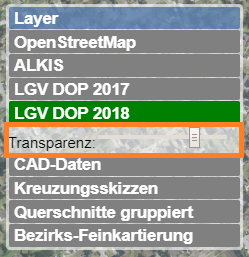
\includegraphics[width=.4\textwidth]{./img/layerbaum.png}
 \caption{Layerbaum}
 \label{img:layerbaum}
\end{figure}

\paragraph{Layerbaum} Mit der Schaltfläche Layer im roten Kasten auf \autoref{img:bearbeitung} können die Hintergrundkarten umgeschaltet werden. Beim Überfahren der Schaltfläche mit der Maus öffnet sich der Layerbaum (\autoref{img:layerbaum}). Durch Klick auf die grauen Schaltflächen wird der Layer aktiviert, mit Klick auf eine grüne Schaltfläche wird der Layer wieder deaktiviert. Außerdem besteht die Möglichkeit, die Transparenz einzelner Layer anzupassen (oranger Kasten). 

\subsubsection{Abschnitte laden}
\paragraph{Abschnitte laden nach Kartenausschnitt}
Die Schaltfläche Abschnitte laden (hellblauer Kasten) lädt alle Straßenabschnitte, die sich im Kartenausschnitt befinden (jedoch maximal 1000) aus der TTSIB.

\paragraph{Suche}
Mit der Suche im violetten Kasten in \autoref{img:bearbeitung} kann nach Straßen gesucht werden. Die Suche ist möglich über Wegenummern, Netzknoten und Straßennamen. Nach dem Klick auf Laden werden die zutreffenden Abschnitte geladen und auf diese gezoomt.

\

\subsubsection{Bearbeitungswerkzeuge}
Mit dem Schaltflächen im braunen Kasten werden die Bearbeitungswerkzeuge gesteuert. Diese werden in einzelnen Abschnitten erläutert.

\begin{itemize}
    \item Querschnitte in \autoref{s:querschnitte}
    \item Aufstellvorrichtungen und Schilder in \autoref{s:schilder}
    \item Straßenausstattung in \autoref{s:straus}
\end{itemize}

\subsubsection{Weitere Tools}
\paragraph{Messen}
Mit der Schaltfläche Messen lässt sich ein Messwerkzeug aktivieren. Mittels einfachen Klick in die Karte können Stützpunkte gesetzt werden, mittel Doppelklick wird die Messung beendet. Beim Wechsel des Werkzeuges oder beim Beginn einer neuen Messung wird die alte Messung gelöscht.

\paragraph{Andere Kartendienste}
Mit den Schaltflächen unten links (grüner Kasten) kann zu anderen Kartenportalen gesprungen werden. Hierbei wird das Kartenzentrum und der Maßstab annährend beibehalten. Die Seite wird in einem neuen Browser-Tab geöffnet. Bei einem weiteren Klick wird dieser Browser-Tab aktualisiert.

\section{Querschnitte bearbeiten}
\label{s:querschnitte}

\subsection{Querschnitte laden}
\subsection{Querschnitte hinzufügen}
\subsection{Attribute ändern}
\subsection{Flächen anpassen}

\section{Aufstellvorrichtungen und Schilder bearbeiten}
\label{s:schilder}

\section{Straßenausstattung bearbeiten}
\label{s:straus}

\end{document}
